\section{Pattern-Driven System Optimizations}
\label{sec:pattern-driven_system_optimizations}

In this section, we demonstrate how the structural visibility enabled by our graph definition unlocks a systematic design space for workflow optimization. We first formalize the pattern as a recurring subgraph $(G' \subseteq G)$ within diverse agentic workflows to identify its inherent system-optimization potential, subsequently mapping these patterns to their corresponding optimization mechanisms. We further organize the optimizations into two complementary paradigms. Section~\ref{sec:execution_level_opt} explores \textit{execution-level optimizations}, where the workflow topology remains fixed while the runtime exploits structural motifs to guide scheduling, memory management, and resource placement. Building upon this, Section~\ref{sec:graph_level_optimizations} investigates \textit{graph-level optimizations}, where the system actively mutates the workflow topology---for example, by pruning dense communication edges or introducing dynamic early-exit conditions---to reduce computational complexity and I/O overhead. We further apply those optimizations on two agentic workflows as case studies, see Appendix \ref{sec:case_study}.



\subsection{Execution-level Optimization}
\label{sec:execution_level_opt}

% ---------------------------------------------------------------------------
\subsubsection{Pattern I: Fan-out and Branching (1-to-K)}
\begin{center}
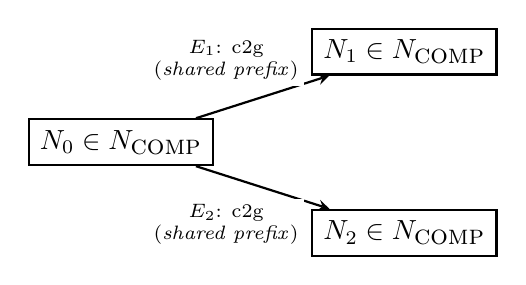
\begin{tikzpicture}[
  node distance=3.6cm,
  >=stealth,
  thick,
  every node/.style={draw, rectangle, inner sep=4pt},
  lab/.style={draw=none, fill=white, inner sep=2pt, font=\scriptsize, align=center} 
]
  \node (n0) {$N_0 \in N_{\textsc{comp}}$};
  \node (n1) [right of=n0, yshift=1.15cm] {$N_1 \in N_{\textsc{comp}}$};
  \node (n2) [right of=n0, yshift=-1.15cm] {$N_2 \in N_{\textsc{comp}}$};

  \draw[->]
    (n0) -- node[pos=0.35, lab, above=6pt, xshift=-6pt]
    {$E_1$: c2g\\(\textit{shared prefix})} (n1);

  \draw[->]
    (n0) -- node[pos=0.35, lab, below=6pt, xshift=-6pt]
    {$E_2$: c2g\\(\textit{shared prefix})} (n2);
\end{tikzpicture}
\end{center}

\paragraph{Structural Description \& System Optimization Potential}
The Fan-out pattern occurs when a single parent node directly spawns multiple parallel child reasoning paths (e.g., expansion in Tree-of-Thought). Structurally, a single computational path abruptly splits into $K$ concurrent paths without an explicit control operator.
\begin{itemize}
    \item \textbf{Extreme Context Redundancy:} Because all $K$ child nodes consume incoming edges directly from $N_0$, their prompts contain a massive, mathematically identical prefix. The theoretical potential here is to reduce the prefill complexity of the children from $\mathcal{O}(K \times \text{Length})$ to $\mathcal{O}(1 \times \text{Length}_{\text{prefix}}) + \mathcal{O}(K \times \text{Length}_{\text{suffix}})$.
    \item \textbf{Concurrency Burst (Prefill Shock):} The sudden topological divergence instantly injects $K$ new computation nodes into the scheduling queue. Scheduled simultaneously, this creates a massive spike in GPU compute demand, theoretically starving any currently active nodes in the decode phase.
\end{itemize}

\paragraph{Applied System Optimizations}
To exploit the context redundancy exposed by the Fan-out pattern, standard LRU caching is inadequate. Systems like \textbf{SGLang (NSDI 2024)}~\citep{zheng2024sglang} perfectly match this potential by maintaining a radix tree of KV cache segments. When $N_1$ and $N_2$ are invoked, the engine performs a longest-prefix match to completely deduplicate the prefill computation of the shared $N_0$ context. Furthermore, to mitigate the ``Prefill Shock,'' workflows fundamentally benefit from stall-free scheduling mechanisms. \textbf{Sarathi-Serve (OSDI 2024)}~\citep{agrawal2024taming} addresses this exact bottleneck by chunking massive parallel prefill requests and interleaving them with active decoding tokens, neutralizing latency spikes without compromising GPU saturation.

% ---------------------------------------------------------------------------
\subsubsection{Pattern II: Fan-in and Aggregation (K-to-1)}

\paragraph{Canonical Graph Definition}
\begin{center}
\begin{tikzpicture}[node distance=3cm, >=stealth, thick]
    \node (n1) [draw, rectangle] {$N_1 \in N_{comp}$};
    \node (n2) [draw, rectangle, below of=n1, node distance=2cm] {$N_2 \in N_{comp}$};
    \node (op) [draw, diamond, aspect=2, right of=n1, below of=n1, node distance=3cm, yshift=1cm] {$Op_{ensemble}$};
    \node (n3) [draw, rectangle, right of=op, node distance=3.5cm] {$N_3 \in N_{comp}$};

    \draw[->] (n1) -- node[above, sloped]{\small $E_1$: g2c} (op);
    \draw[->] (n2) -- node[midway, sloped, below=12pt, draw=none, font=\scriptsize, inner sep=1pt] {$E_2$: g2c} (op);
    \draw[->] (op) -- node[above]{\small $E_3$: c2g} (n3);
\end{tikzpicture}
\end{center}

\paragraph{Structural Description \& System Optimization Potential}
The Fan-in pattern represents a topological synchronization point. Multiple independent upstream branches converge at an $Op_{ensemble}$ operator (e.g., majority voting, debate synthesis) before downstream execution can proceed.
\begin{itemize}
    \item \textbf{Strict Synchronization Barrier:} The execution of $Op_{ensemble}$ cannot commence until the final token of the slowest upstream branch ($N_{slowest}$) is generated. The optimization potential lies in compressing the latency variance among upstream nodes; any straggler directly translates to idle GPU memory residency for the branches that finish early but must wait at the barrier.
\end{itemize}

\paragraph{Applied System Optimizations}
Because the synchronization barrier is an explicit topological construct, the runtime can proactively manage tail latency risks. \textbf{Parrot (OSDI 2024)}~\citep{lin2024parrot} utilizes a DAG-aware executor that tracks critical paths leading to aggregation operators. By identifying the Fan-in structure, the scheduler dynamically elevates the priority of straggling branches. This objective-driven scheduling ensures parallel branches reach the $Op_{ensemble}$ synchronously, minimizing idle memory waste at the join barrier.


% ---------------------------------------------------------------------------
\subsubsection{Pattern III: Iterative Reflection (Self-Cycle)}

\paragraph{Canonical Graph Definition}
\begin{center}
\begin{tikzpicture}[node distance=4cm, >=stealth, thick]
    \node (n1) [draw, rectangle] {$N_1 \in N_{comp}$};
    \node (op) [draw, diamond, aspect=2, right of=n1] {$Op_{eval}$};

    \draw[->] (n1.east) -- node[above]{\small $E_1$: g2c} (op.west);
    \draw[->] (op.north) -- ++(0,1) -| node[above, pos=0.25]{\small $E_2$: c2g (feedback)} (n1.north);
\end{tikzpicture}
\end{center}

\paragraph{Structural Description \& System Optimization Potential}
The Iterative Reflection pattern features a direct back-edge governed by an $Op_{eval}$ node, modeling an agent critiquing and refining its own output. Topologically, this forms a self-cycle on a single computation node.
\begin{itemize}
    \item \textbf{High Temporal Locality of Base Prompts:} Despite the dynamic growth of the context with each appended critique, the foundational system prompt and instruction set of $N_1$ remain mathematically invariant across every traversal of the back-edge.
\end{itemize}

\paragraph{Applied System Optimizations}
To address the extreme temporal locality across back-edges, systems like \textbf{Pie (SOSP 2025)}~\citep{gim2025pie} introduce programmable KV cache control. This aligns perfectly with the Self-Cycle pattern by allowing the application to explicitly ``pin'' the stable KV pages of $N_1$ in GPU memory. Pinning prevents standard recency-based (LRU) eviction policies from discarding critical context between iterative refinement steps, effectively reducing prefill latency to near-zero for subsequent loop traversals.

% ---------------------------------------------------------------------------
\subsubsection{Pattern IV: Centralized Routing (Star Topology)}

\paragraph{Canonical Graph Definition}
\begin{center}
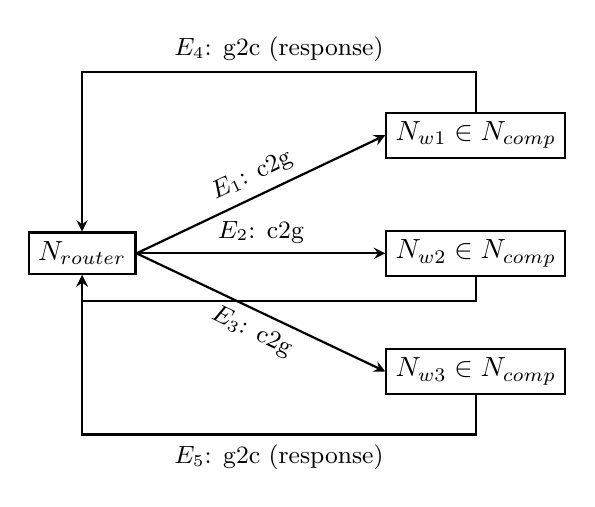
\begin{tikzpicture}[>=stealth, thick]
    \node (n_router) [draw, rectangle] at (0, 0) {$N_{router}$};
    \node (n_w1) [draw, rectangle] at (5, 1.5) {$N_{w1} \in N_{comp}$};
    \node (n_w2) [draw, rectangle] at (5, 0) {$N_{w2} \in N_{comp}$};
    \node (n_w3) [draw, rectangle] at (5, -1.5) {$N_{w3} \in N_{comp}$};

    \draw[->] (n_router.east) -- node[above, sloped]{\small $E_1$: c2g} (n_w1.west);
    \draw[->] (n_router.east) -- node[above]{\small $E_2$: c2g} (n_w2.west);
    \draw[->] (n_router.east) -- node[below, sloped]{\small $E_3$: c2g} (n_w3.west);
    
    \draw[->] (n_w1.north) -- ++(0,0.5) -| node[above, pos=0.25]{\small $E_4$: g2c (response)} (n_router.north);
    \draw[->] (n_w2.south) -- ++(0,-0.3) -| (n_router.south);
    \draw[->] (n_w3.south) -- ++(0,-0.5) -| node[below, pos=0.25]{\small $E_5$: g2c (response)} (n_router.south);
\end{tikzpicture}
\end{center}

\paragraph{Structural Description \& System Optimization Potential}
This pattern occurs when a centralized router node directly dispatches tasks to specific specialist workers and re-aggregates their responses. Structurally, it forms a star topology with direct fan-outs to multiple workers and converging back-edges.
\begin{itemize}
    \item \textbf{Asymmetric Workload Inflation:} Because $N_{router}$ is visited on every cycle and acts as the central aggregator, its context window (e.g., global conversation history) grows monotonically. The structural asymmetry is stark: $N_{router}$ rapidly becomes heavily prefill-bound, while downstream worker nodes generate highly localized responses and remain decode-bound.
\end{itemize}

\paragraph{Applied System Optimizations}
Identifying the asymmetric prefill vs. decode bottleneck via the Star topology maps the workflow naturally onto disaggregated architectures, such as \textbf{Splitwise (ISCA 2024)}~\citep{patel2024splitwise} and \textbf{DistServe (OSDI 2024)}~\citep{zhong2024distserve}. By routing the prefill-heavy $N_{router}$ executions to compute-optimized instances and the decode-heavy worker tasks to memory-optimized instances, the system prevents the router's monotonic context growth from degrading overall cluster throughput.

% ---------------------------------------------------------------------------
\subsubsection{Pattern V: Heterogeneous Interleaving (Compute-I/O Alternation)}

\paragraph{Canonical Graph Definition}
\begin{center}
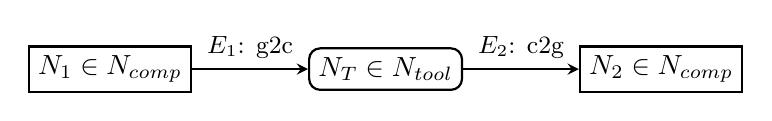
\begin{tikzpicture}[node distance=3.5cm, >=stealth, thick]
    \node (n1) [draw, rectangle] {$N_1 \in N_{comp}$};
    \node (nt) [draw, rectangle, right of=n1, rounded corners] {$N_T \in N_{tool}$};
    \node (n2) [draw, rectangle, right of=nt] {$N_2 \in N_{comp}$};

    \draw[->] (n1) -- node[above]{\small $E_1$: g2c} (nt);
    \draw[->] (nt) -- node[above]{\small $E_2$: c2g} (n2);
\end{tikzpicture}
\end{center}

\paragraph{Structural Description \& System Optimization Potential}
The Heterogeneous Interleaving pattern occurs when LLM reasoning nodes frequently yield to external tool executions (e.g., Code Interpreters, Web Search). Topologically, this creates an alternating sequence of $N_{comp}$ and $N_{tool}$ nodes, explicitly bridged by cross-device data transfers ($g2c$ and $c2g$).
\begin{itemize}
    \item \textbf{Severe GPU Memory Underutilization:} When the workflow traverses the $E_1$ ($g2c$) edge to enter $N_T$, GPU execution halts. Tool execution latency is typically unbounded and highly unpredictable. If the runtime obliviously holds $N_1$'s massive KV cache in the GPU during $N_T$'s execution, that memory becomes ``dead weight,'' drastically reducing the cluster's effective batch size.
    \item \textbf{Perfect Resource Decoupling:} The explicit topological distinction between $N_{comp}$ and $N_{tool}$ signals an absolute resource decoupling. $N_T$ requires zero Tensor Core utilization, providing the scheduler with a deterministic window to yield GPU compute.
\end{itemize}

\paragraph{Applied System Optimizations}
The transition to an $N_{tool}$ node serves as a perfect structural trigger for memory offloading. While \textbf{vLLM (SOSP 2023)}~\citep{kwon2023efficient} originally designed its KV cache swapping mechanism as a reactive measure to handle out-of-memory preemption, the $G=(N, E, Op)$ graph allows the scheduler to use this mechanism \textit{proactively}. Upon traversing the $E_{g2c}$ edge, the runtime can immediately swap out the workflow's KV cache and yield the GPU to other active agents. To fully exploit this resource decoupling, \textbf{Parrot (OSDI 2024)}~\citep{lin2024parrot} models non-LLM steps as Semantic Variables within a unified dataflow graph. When an $N_{tool}$ node executes, Parrot's DAG-aware executor dispatches it to asynchronous CPU/I/O worker pools, guaranteeing the GPU engine remains entirely focused on $N_{comp}$ nodes from concurrent workflows.


\subsection{Graph-Level Optimizations}
\label{sec:graph_level_optimizations}

Graph-level optimization modifies the structure of an existing workflow by leveraging the graph formalism defined in the preceding sections. Unlike execution-level techniques that preserve topology, graph-level methods restructure the computation graph to reduce the number of agent invocations, the amount of inter-agent communication, or the amount of active model compute. We focus on four representative strategies: (1)~adaptive subgraph pruning via early-exit conditions, (2)~heterogeneous node downscaling by replacing large models with smaller task-specialized ones, (3)~sparse expert decomposition through router--expert subgraphs, and (4)~subgraph consolidation that collapses multi-agent pipelines into single-model invocations. Additional technical details and extended literature discussion are deferred to Appendix~\ref{app:graph_level_optimizations_extended}.

\subsubsection{Strategy I: Adaptive Subgraph Pruning (Early Exits)}

\paragraph{Canonical Graph Transformation.}
Consider a sequential workflow
\[
N_0 \xrightarrow{E_1} N_1 \xrightarrow{E_2} \cdots \xrightarrow{E_k} N_k
\]
where each $N_i \in \mathcal{N}_{\text{comp}}$ is an LLM-based reasoning node. Adaptive Subgraph Pruning inserts lightweight exit operators $\text{Op}_{\text{exit}}$ after selected nodes:
\[
N_0 \rightarrow \text{Op}_{\text{exit}}^{(0)} \rightarrow
\left\{
\begin{array}{ll}
\texttt{return} & \text{if } \text{conf}(N_0) \geq \tau \\
N_1 \rightarrow \cdots & \text{otherwise}
\end{array}
\right.
\]
and similarly at later depths. If the exit condition is met, all downstream nodes are pruned from the active execution graph.

\paragraph{Structural Description and System Optimization Potential.}
This pattern exploits the fact that many queries do not require the full depth of a multi-agent pipeline. Early exit reduces latency by skipping downstream LLM calls, lowers token costs by avoiding prompt growth across later stages, and reclaims memory by eliminating KV-cache allocation for pruned nodes. In agentic workflows with cumulative context, these savings can be especially pronounced because later agents often consume all prior outputs. Prior work on adaptive computation, LLM cascades, and difficulty-aware workflow selection supports the same principle: computational depth should scale with input difficulty. We therefore view adaptive pruning as the graph-level analogue of model-level early exit and API-level routing. Further examples and discussion are provided in Appendix~\ref{app:graph_level_optimizations_extended}.

\subsubsection{Strategy II: Heterogeneous Node Downscaling}
\label{sec:centralized_routing}

\paragraph{Canonical Graph Transformation.}
Let a workflow graph $G = (\mathcal{N}, \mathcal{E}, \text{Op})$ initially assign the same large model $\mathcal{M}_{\text{large}}$ to every computation node:
\[
G_{\text{homo}} =
\{N_0^{\mathcal{M}_{\text{large}}}, \ldots, N_k^{\mathcal{M}_{\text{large}}}\}
\;\longrightarrow\;
G_{\text{hetero}} =
\{N_0^{\mathcal{M}_{\text{large}}}, N_1^{\mathcal{M}_{\text{small}}^{(1)}}, \ldots, N_k^{\mathcal{M}_{\text{small}}^{(k)}}\}.
\]
Here, selected nodes are replaced with smaller task-specialized models while preserving the graph topology.

\paragraph{Structural Description and System Optimization Potential.}
This strategy addresses the mismatch between the broad capabilities of frontier models and the narrow functional roles of many agents. In practice, nodes such as summarizers, formatters, verifiers, or tool-call generators often do not require a uniformly large backend. Replacing them with smaller specialized models reduces per-node FLOPs, lowers memory usage, and enables more efficient serving and fine-tuning. The key systems insight is that once the workflow is represented explicitly as a graph, each node can be assigned the smallest model sufficient for its role. Empirical work on distillation, SLM-based agents, and heterogeneous multi-agent systems suggests that such right-sizing can preserve and sometimes improve end-to-end performance while sharply lowering cost. Additional evidence and examples are included in Appendix~\ref{app:graph_level_optimizations_extended}.

\subsubsection{Strategy III: Sparse Expert Decomposition}

\paragraph{Canonical Graph Transformation.}
Consider a dense computation node $N_i$ instantiated with a single model $\mathcal{M}_{\text{dense}}$. Sparse Expert Decomposition replaces it with a router plus a set of specialized experts:
\[
N_i^{\mathcal{M}_{\text{dense}}}
\;\longrightarrow\;
\bigl\{
N_{\text{router}}^{\mathcal{R}},
N_{e_1}^{\mathcal{E}_1},
\ldots,
N_{e_n}^{\mathcal{E}_n}
\bigr\},
\]
where the router activates only a small subset of experts for each query, followed by an aggregation step before passing outputs to downstream nodes.

\paragraph{Structural Description and System Optimization Potential.}
This transformation lifts the mixture-of-experts idea from the layer level to the workflow level. Instead of applying the same generalist agent to all inputs, the workflow dispatches each query to only the relevant expert subgraph. The result is sparse activation at the agent level, improved specialization, and more flexible placement across hardware tiers. Conceptually, the router becomes a scheduling primitive: it not only selects capabilities but also determines where computation should run. Recent work on MoE models, adaptive operator selection, and query-dependent workflow sampling shows that activating only a subset of experts can reduce cost while preserving or improving quality. Extended discussion appears in Appendix~\ref{app:graph_level_optimizations_extended}.

\subsubsection{Strategy IV: Subgraph Consolidation}

\paragraph{Canonical Graph Transformation.}
Let $G_{\text{sub}} = (\mathcal{N}_{\text{sub}}, \mathcal{E}_{\text{sub}})$ be a connected multi-agent subgraph. Subgraph Consolidation collapses it into a single node:
\[
G_{\text{sub}} =
\bigl(\{N_{i_1}^{\mathcal{M}_1}, \ldots, N_{i_m}^{\mathcal{M}_m}\}, \mathcal{E}_{\text{sub}}\bigr)
\;\longrightarrow\;
N_{\text{consolidated}}^{\mathcal{M}_{\text{large}}}.
\]
All internal edges are removed, and external edges are rewired to the consolidated node.

\paragraph{Structural Description and System Optimization Potential.}
This strategy is motivated by the observation that multi-agent workflows, especially homogeneous ones, may incur coordination overhead without proportional quality gains. Consolidation removes inter-agent communication, reduces context fragmentation across stages, and prevents error propagation through intermediate hand-offs. In serving terms, it replaces many small invocations with one longer inference that can better exploit cache reuse and long-context reasoning. Recent results suggest that some homogeneous multi-agent workflows can be simulated or distilled into single-model executions with similar or better performance. However, consolidation is most appropriate when the relevant functions fit within one model’s capability and context window. We discuss these boundary conditions further in Appendix~\ref{app:graph_level_optimizations_extended}.

\paragraph{Summary.}
Taken together, these four transformations show that once an agentic system is exposed as a graph, optimization need not be limited to faster execution of a fixed topology. The graph itself becomes the optimization surface: it can be shortened through pruning, right-sized through heterogeneous model assignment, sparsified through expert decomposition, or collapsed through consolidation. This graph-centric view enables runtimes to move beyond worst-case static workflows and instead construct execution paths that better match the structure and difficulty of each query. Additional formal detail, systems interpretation, and literature coverage are provided in Appendix~\ref{app:graph_level_optimizations_extended}.



